\documentclass{standalone}
\usepackage{tikz}
\standaloneenv{tikzpicture}
\usetikzlibrary{arrows}
\tikzset{%
 >=stealth'
}
\newenvironment{localtoimage}[3][]{%
 \node (I) [inner sep=0pt] {\includegraphics[#3]{#2}};%
 \begin{localto}[#1]{I}%
}{%
 \end{localto}%
}
\newenvironment{localto}[2][]{
 \path let \p1=(#2.center), \p2=(#2.north), \p3=(#2.east) in coordinate (#2X) at (\x3-\x1,0) coordinate (#2Y) at (0,\y2-\y1);
 \begin{scope}[x={(#2X)}, y={(#2Y)}, shift={(#2.center)},#1]
}{
 \end{scope}
}
\newcommand*{\ExtractCoordinateOld}[1]{%
 \path [transform canvas] (#1);
 \pgfgetlastxy{\XCoord}{\YCoord}%
}

\usepackage{substr}
% \def\jobname{dark}
\IfSubStringInString{\detokenize{dark}}{\jobname}{
%  \pagecolor{black}
 \def\fg{white}
 \def\bg{black}
 \color{\fg}
}{
 \def\fg{black}
 \def\bg{white}
}

\usetikzlibrary{calc, spy}
\begin{document}
\begin{tikzpicture}[remember picture]
 \begin{scope}[spy using outlines={size=2 cm, connect spies, magnification=5, circle}]
  \begin{localtoimage}{distributions}{width=.5\textwidth}
   \def\dx{.1}
   \coordinate (r) at ($(I.east)+(\dx,0)$);
   \coordinate (l) at ($(I.west)-(\dx,0)$);
   \foreach \n/\c/\a/\f in {C/r/south west/complex,
                            L/r/north west/lures,
                            T/l/south east/traps,
                            S/l/north east/simple} {
    \node (\n) at (\c) [anchor=\a]{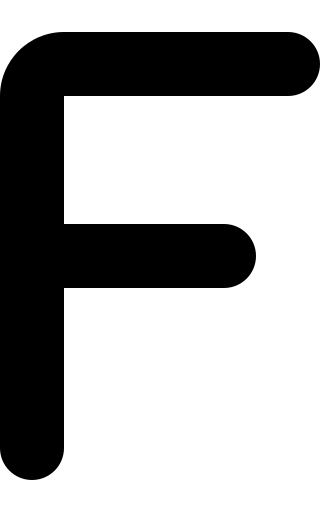
\includegraphics[width=.2\textwidth]{example_\f.png}};
   }

   \foreach \n/\x/\y/\c in {C/.633/.646/0173b2,
                            L/.643/-.493/de8f05,
                            T/-.106/.021/029e73,
                            S/-.512/-.677/d55e00} {
    \definecolor{tmp}{HTML}{\c}
    \draw [dashed, tmp] (\n) -- (\x, \y);
%     \draw [thin, red] (\x, 1) -- (\x, -1) (1, \y) -- (-1, \y);
   }
  \end{localtoimage}

  \foreach \c/\a/\b in {C/{-.9,.9}/{.25, -.25},
                        L/{.95,-.95}/{-.25, .25},
                        T/{.95,-.3}/{-.25, .25}} {
   \ExtractCoordinateOld{$(\c)+(\a)$}
   \edef\tmp{\noexpand\spy [red] on (\XCoord, \YCoord) in node at ($(\c)+(\b)$);}
   \tmp
  }

%   \spy [red] on ($(C)+(-.9,.9)$) in node at ($(C)+(.25, -.25)$);
%   \spy [red] on ($(L)+(.95,-.95)$) in node at ($(L)+(-.25, .25)$);
%   \spy [red] on ($(T)+(.95,-.3)$) in node at ($(T)+(-.25, .25)$);
\end{scope}
\end{tikzpicture}
\end{document}
